\chapter{Introduction}
\section{Overview}
%https://nsdsguidelines.paris21.org/node/291
%https://papers.ssrn.com/sol3/papers.cfm?abstract_id=2622220


%markets:
%https://link.springer.com/article/10.1007/s10551-010-0402-8
%https://www.oecd-ilibrary.org/content/paper/5k49dfg9fb6d-en

%problem statement
Almost two billion people live in Fragile States \todo{cite}. These fragile states are characterized by weak state capacity, leaving its citizens vulnerable to various shocks, and unable to the benefit from the growing world wide prosperity. \todo{expand: why do we care?}

The key factor that sets apart Fragile States from their more stable counterparts, is the institutional environment \citep{Rodrik2004,Acemoglu2000}. This term is used to describe the rules and norms that shape (economic) life. It covers crucial things such as protection of property rights and equal treatment by the law \citep{Acemoglu2005}. Such good institutions  foster development by incentivizing innovation. However, the relationship between institutions and development does not run in one direction. While institutions cause growth \citep{Acemoglu2000}, the economic growth that accompanies development also allows for better institutions. It is possible that countries could enter a virtuous cycle, where improved institutional quality enhances growth, which improves institutional quality \citep{Voors2011}.

%
Social capital is closely related to institutions. \todo{what is social capital?} Especially in poorer countries, social capital plays an important role in facilitating economic activity \citep{Knack1997}. In such countries, social capital may be a substitute for formal institutions by providing insurance and securing property rights. To a large extent, such social capital is underpinned by pro-social behaviour. \todo{really?}

%However, institutions can also increase cooperative behaviour \citep{Bo2008,Henrich2010}. 

This implies that countries with a high level of social capital or good institutions can enter a virtuous cycle of institutions producing growth and social capital; and social capital and growth producing quality institutions. The question on how to enable such a virtuous cycles for fragile states is too large for any one thesis. This thesis aims to provide empirical, micro-level level evidence on how social capital and behaviour mediate development in fragile states. Figure \ref{fig:intro_framework} outlines these concepts. Each chapter in this thesis then explores one subset of the possible relationships within the framework.

I focus on three separate characteristics of Fragile States, that either present risks or opportunities for their development. Firstly, they are frequently settings for violent conflict. SOME STATISTICS MAYBE? Secondly, they are poorly connected to world markets. This leads to a lack of opportunities for exchange and specialization, and underwhelming economic development. Thirdly, Fragile States are large recipients of development aid. The lack of state capacity makes it hard to fulfil citizen's needs for healthcare, education, and services, leading to international donors to attempt and alleviate the resulting humanitarian crises.

\begin{figure}[htb]
  \centering
  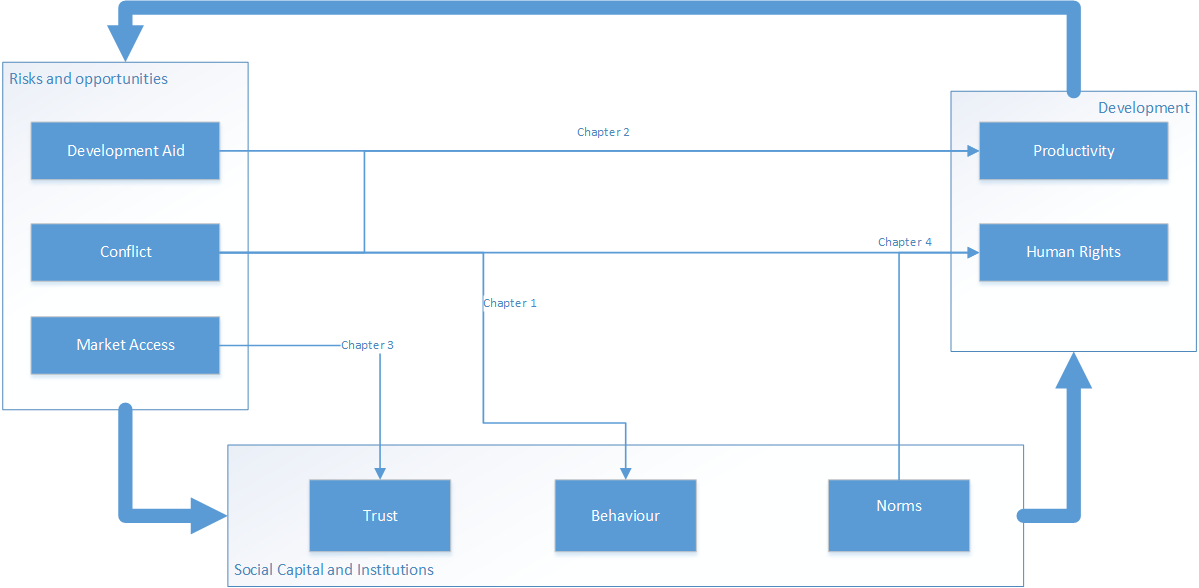
\includegraphics[width=0.8\linewidth]{"C:/Users/Koen/Documents/GitHub/thesis/figures/introduction/conceptual_framework.png"}
  \caption{Conceptual Framework}
  \label{fig:intro_framework}
\end{figure}

As for development, I focus on agricultural productivity and human rights. Agricultural productivity is seen as a necessary precondition for further, economy-wide, productivity improvements. \todo{why?} However, a focus on productivity is too narrow to fully capture the problems that life in fragile states presents in terms of development.   Productivity gains mean little in the face of flagrant human rights violations.

The questions this thesis aims to answer are:
\begin{enumerate}
	\item What is the relationship between conflict and competitive behaviour? (Chapter \ref{chap:slfootball});
	\item What is the effect of input subsidies on novel technology adoption? (Chapter \ref{chap:n2a_impact});
	\item What is the effect of market access on trusting behaviour (Chapter \ref{chap:cameroontrust}); and,
	\item What are the drivers of sexual and gender-based violence in Eastern Congo (Chapter \ref{chap:congogbv}).
\end{enumerate}

\section{Contribution}
The primary contribution of this thesis lies in the collection of large-scale datasets in fragile states. This fits within a broader trend where the amount of data collected in such states has increased over the past decades. Two factors contribute to this increase. On the supply side, cost of data collection is dropping. Information technology allows for cheaper collection and processing of data, and for more effective monitoring of field staff. On the demand side, is a drive to more rigorously evaluate the impact development aid. This necessitates the collection of detailed household-level data to compare project beneficiaries with non-beneficiaries. The primary funding for this PhD-thesis comes from such an evaluation: the MFS II evaluations, commissioned by the Dutch ministry of foreign affairs.

Despite this increase in data collection efforts, citizens of Fragile States remain under-represented in studies on behaviour. Chapter \ref{chap:slfootball} contributes by studying the effects of conflict on youth in Sierra Leone. Chapter \ref{chap:cameroontrust} contributes to this by collecting large-scale data on behaviour of an understudied group: Africans from rural areas, with poor access to markets. Chapter 4 studies the dynamics of sexual violence in Congo. Despite the prominence the topic has had in public discourse on Congo, and despite its severity, little data exists on these dynamics. This is partly due the difficulties and costs inherent in operating in unstable countries.

All data sets used for analyses, and all protocols and analysis scripts are released to the public domain.


\section{Outline}


%bibliography, this is needed for bibtex
\clearpage 
\bibliographystyle{chicago}
%path to .bib file (e.g. automatically exported by mendeley) DO NOT include the file extension!
\bibliography{C:/Users/Koen/Dropbox/Literatuur/Mendeley/Bibtex/Thesis-Introduction}